\documentclass[11pt]{article}

\usepackage[T1]{fontenc}
\usepackage[utf8]{inputenc}
\usepackage{lmodern}
\usepackage{microtype}
\usepackage{amsmath,amssymb,bm}
\usepackage{amsthm}
\usepackage{graphicx}
\usepackage{booktabs}
\usepackage{array}
\usepackage{geometry}
\usepackage{setspace}
\usepackage{float}
\usepackage{algorithm}
\usepackage{algpseudocode}
\usepackage[colorlinks=true,linkcolor=blue,urlcolor=blue,citecolor=blue]{hyperref}
\usepackage[font=small,labelfont=bf]{caption}
\graphicspath{{figures/}}

\geometry{margin=1in}
\setstretch{1.12}

\newcommand{\ESS}{\mathrm{ESS}}
\newcommand{\NegBin}{\operatorname{NegBin}}
\algnewcommand\algorithmicforeach{\textbf{for each}}
\algdef{S}[FOR]{ForEach}[1]{\algorithmicforeach\ #1\ \textbf{do}}

\newtheorem{theorem}{Theorem}
\newtheorem{proposition}[theorem]{Proposition}

\title{EpiSurveil: A Modular Python Framework for Epidemic\\
       Surveillance, Sequential Bayesian Estimation, and\\
       Particle-Filter-Guided Optimal Intervention Planning}
\author{Florent Ouabo Kamkumo}
\date{\today}

\begin{document}
\maketitle

%% -----------------------------------------------------------------------
\begin{abstract}
\textbf{Background:}
Linking mechanistic epidemic models to heterogeneous surveillance data
streams in real time, and translating the resulting estimates into
actionable intervention recommendations, requires software that integrates
disease dynamics, observation models, sequential inference, and
decision logic in a coherent and testable manner.
Existing tools address individual layers but rarely combine all four.

\textbf{Methods:}
We present \texttt{EpiSurveil}, an open-source Python platform that integrates
(i) a nine-compartment SVEAIHCRD model with multipatch force of infection,
(ii) a Bootstrap Particle Filter (BPF) with systematic resampling and
     tempered multi-channel likelihoods tracking five time-varying parameters
     jointly with the epidemic state,
(iii) a reporting-delay convolution pipeline for case-channel alignment,
(iv) a SARI-sentinel panel-extension methodology that extrapolates
     hospitalisation surveillance beyond mandatory reporting periods, and
(v) a two-control optimal intervention module combining
    non-pharmaceutical intervention intensity $u_t$ with testing/detection
    intensity $v_t$, solved via direct transcription (L-BFGS-B) for
    single-horizon planning and via Particle-Filter Model Predictive
    Control (PF-MPC) for adaptive receding-horizon decision support.

\textbf{Results:}
Applied to German COVID-19 data (10~March~2020 to 7~October~2024;
1\,673 days extended with RKI COVID-SARI sentinel data),
the five-parameter BPF ($N=2\,000$ particles;
dynamic $\beta_t$, $\tau_{I,t}$, $\delta_{H,t}$, $\rho_{C,t}$, $Q_{C,t}$)
achieves case-channel 80\,\% coverage of 94.9\,\%, ICU 70.1\,\%, and
mean ESS~$=1\,259$.
The two-control optimiser converges in under 20~seconds for a 90-day horizon
(180 variables); PF-MPC over a 60-day retrospective period with a
14-day lookahead runs in~$\sim$17~seconds and averts 1\,430 deaths
relative to an uncontrolled baseline.

\textbf{Conclusions:}
\texttt{EpiSurveil} provides a transparent, modular foundation for
multi-source epidemic data assimilation and uncertainty-aware intervention
planning.
Its layered design allows components to be replaced independently, supporting
both methodological research and operational public health applications.
\end{abstract}

\noindent\textbf{Keywords:}
epidemic surveillance; particle filter; Bayesian data assimilation;
optimal control; model predictive control; COVID-19; testing strategy;
non-pharmaceutical interventions; SVEAIHCRD.


%% -----------------------------------------------------------------------
\section{Introduction}
\label{sec:intro}
%% -----------------------------------------------------------------------

Real-time epidemic surveillance combines latent biological processes with
delayed, over-dispersed, and heterogeneous observations.
Mechanistic compartmental models translate epidemiological assumptions into
interpretable population states \cite{anderson1991,keeling2008}, but coupling
them to data in real time requires non-Gaussian, non-linear filtering methods.
Sequential Monte Carlo (particle filtering) approximates the resulting
filtering distribution without linearisation or Gaussian assumptions
\cite{gordon1993,doucet2001,chopin2020}, making it well suited to epidemic
state-space models with time-varying parameters and mixed-integer data.

Once a filtered state estimate is available, a natural second question arises:
what intervention should be applied today, given current uncertainty about the
epidemic state and parameter values?
Optimal epidemic control has been studied analytically for simple SIR dynamics
\cite{bolzoni2017,bliman2021}, but operational tools that close the
loop between a running particle filter and a real-time controller remain scarce.

Existing frameworks address individual modelling layers.
POMP \cite{ionides2006,king2016} provides likelihood-based inference for
partially observed Markov processes in R.
EpiEstim \cite{cori2013} and EpiNow2 \cite{abbott2020} focus on real-time
$R_t$ estimation with explicit reporting-delay models.
Bayesian evidence synthesis frameworks \cite{birrell2021} jointly assimilate
multiple data streams in a batch setting.
Semi-mechanistic regression models \cite{flaxman2020,brauner2021} have
estimated intervention effects across countries.
None of these integrates online sequential inference, multi-channel
observation models, and uncertainty-aware adaptive control in a single
testable Python package.

\texttt{EpiSurveil} fills this gap.
Its design separates six independently testable layers:
(i) epidemic dynamics, (ii) stochastic simulation backends,
(iii) observation likelihoods with reporting delays,
(iv) sequential Bayesian inference,
(v) single-horizon two-control optimal intervention, and
(vi) particle-filter model predictive control (PF-MPC).
Each layer has a well-defined interface and is covered by unit tests
so components can be substituted without breaking surrounding code.

The platform is validated on four years of German COVID-19 surveillance,
extended through October~2024 using RKI COVID-SARI sentinel hospitalisation
data, using a SVEAIHCRD model with five jointly tracked time-varying
parameters and a tempered multi-channel likelihood.


%% -----------------------------------------------------------------------
\section{Mathematical framework}
\label{sec:math}
%% -----------------------------------------------------------------------

\subsection{SVEAIHCRD compartment model}
\label{sec:model}

Let $x(t)=(S,V,E,A,I,H,C,R,D)^{\!\top}$ denote the population compartments:
Susceptible, Vaccinated (single combined compartment with vaccine efficacy
$\varepsilon$), Exposed, Asymptomatic infectious, Symptomatic infectious,
Hospitalised (general ward), Critical (ICU), Recovered, and Dead.
The continuous-time dynamics are governed by
\[
  \dot{x}(t) = f\!\bigl(x(t);\,\vartheta(t)\bigr),
\]
where $\vartheta(t)$ collects the model parameters, five of which vary
with time (Section~\ref{sec:dynamic}).  The core transition rates are:

\begin{align}
\text{Force of infection:}\quad
  \lambda(t) &= \beta_t\,\frac{I(t)+\eta_A A(t)}{N_{\mathrm{living}}(t)},
  \label{eq:foi}\\
\text{Vaccination:}\quad
  S &\xrightarrow{\nu} V \xrightarrow{\omega_V} S, \nonumber \\
\text{Infection:}\quad
  S &\xrightarrow{\lambda}\,,\quad
  V \xrightarrow{(1-\varepsilon)\lambda} \to E, \nonumber \\
\text{Progression:}\quad
  E &\xrightarrow{\sigma}
    \begin{cases} A & \text{prob.\ } 1-\kappa \\ I & \text{prob.\ } \kappa \end{cases},
  \nonumber \\
\text{Hospitalisation:}\quad
  I &\xrightarrow{\tau_{I,t}} H \xrightarrow{\tau_H} C, \nonumber \\
\text{Recovery/death:}\quad
  A,I &\xrightarrow{\gamma_{A,I}} R;\quad
  H \xrightarrow{\delta_{H,t}} D;\quad
  C \xrightarrow{\delta_C} D. \nonumber
\end{align}

The living population $N_{\mathrm{living}}=S+V+E+A+I+H+C+R$ decreases only
through deaths $\delta_{H,t}H+\delta_C C$.
Positivity and mass balance are enforced by non-negativity projection after
each Euler step.

\subsection{Multipatch force of infection}
\label{sec:multipatch}

For $P$ geographic patches with state matrices
$\bm{X}\in\mathbb{R}^{P\times 9}$, a mobility matrix
$\bm{M}\in\mathbb{R}^{P\times P}$ ($M_{pq}$ = fraction of time patch-$p$
residents spend in patch $q$), and patch-level transmission rates
$\bm{\beta}\in\mathbb{R}^P$, the force of infection on patch $p$ is
\begin{equation}
  \lambda_p = \beta_p \sum_q M_{pq}\,
  \frac{I_q + \eta_A A_q}{N_{\mathrm{living},q}}.
  \label{eq:multipatch}
\end{equation}
Equation~\eqref{eq:multipatch} is implemented in
\texttt{models/multipatch.py} and tested for dimensional consistency
and non-negativity.

\subsection{Five dynamic parameters as log-random walks}
\label{sec:dynamic}

Five parameters evolve as independent, bounded log-random walks:
\begin{equation}
  \theta_t = \bigl(\beta_t,\;\tau_{I,t},\;\delta_{H,t},\;\rho_{C,t},\;Q_{C,t}\bigr),
\end{equation}
where $\beta_t$ is the transmission rate, $\tau_{I,t}$ the daily
hospitalisation rate from $I$, $\delta_{H,t}$ the in-hospital case fatality
rate, $\rho_{C,t}$ the ICU fraction of the hospitalised cohort, and
$Q_{C,t}$ the symptomatic case detection (reporting) probability.
Each satisfies
\begin{equation}
  \log\theta_{t+1}^{(k)} = \mathrm{clip}\!\bigl(
    \log\theta_t^{(k)} + \sigma_k\,\eta_t^{(k)},\;
    \log\theta_{\min}^{(k)},\;\log\theta_{\max}^{(k)}\bigr),
  \quad \eta_t^{(k)}\overset{\mathrm{iid}}{\sim}\mathcal{N}(0,1),
  \label{eq:logRW}
\end{equation}
with $\sigma_\beta=0.040$ (transmission responds to daily behavioural
and variant changes),
$\sigma_{\tau_I}=\sigma_{\delta_H}=\sigma_{\rho_C}=0.018$
(severity shifts on weekly-to-monthly timescales), and
$\sigma_{Q_C}=0.018$ (detection capacity changes slowly).
$Q_{C,t}$ is clipped to $[0.20,\,0.99]$ to prevent degeneracy at very low
or saturated detection.

These five log-random-walk parameters are appended to the nine compartment
states, giving an augmented particle state of dimension $d=14$.

\subsection{Observation model and tempered likelihood}
\label{sec:obs}

Four surveillance channels are observed each day.  The case reporting
probability $Q_{C,t}$ is now the fifth dynamic parameter rather than a fixed
constant, allowing the filter to jointly infer detection changes alongside
the epidemic trajectory:
\begin{align}
  Y_t^{\mathrm{case}}
    &\sim \NegBin\!\bigl(\mu_t^{\mathrm{case}},\,\phi_c\bigr),
  &\mu_t^{\mathrm{case}}
    &= Q_{C,t}\,\kappa\,\sigma\,E_t\;(\text{delay-convolved}), \label{eq:obs_case}\\
  Y_t^{\mathrm{ICU}}
    &\sim \NegBin\!\bigl(\mu_t^{\mathrm{ICU}},\,\phi_{\mathrm{ICU}}\bigr),
  &\mu_t^{\mathrm{ICU}}
    &= C_t, \label{eq:obs_icu}\\
  Y_t^{\mathrm{death}}
    &\sim \NegBin\!\bigl(\mu_t^{\mathrm{death}},\,\phi_D\bigr),
  &\mu_t^{\mathrm{death}}
    &= \delta_{H,t}\,H_t + \delta_C\,C_t, \label{eq:obs_death}\\
  Y_t^{\mathrm{hosp}}
    &\sim \NegBin\!\bigl(\mu_t^{\mathrm{hosp}},\,\phi_H\bigr),
  &\mu_t^{\mathrm{hosp}}
    &= \tau_{I,t}\,I_t\times\mathrm{LOS}. \label{eq:obs_hosp}
\end{align}
Here $\mathrm{LOS}=8$~days is the assumed mean hospital length of stay, and
$\phi_c=80$, $\phi_{\mathrm{ICU}}=12$, $\phi_D=10$, $\phi_H=15$ are the
negative-binomial dispersions.

The joint log-likelihood increment for particle $i$ at step $t$ is
\begin{equation}
  \ell_t^{(i)} = \sum_{k\in\mathcal{A}_t}
    \alpha_k \cdot
    \log p_{\mathrm{NB}}\!\bigl(Y_t^{(k)}\mid\mu_t^{(k),(i)},\phi_k\bigr),
  \label{eq:loglik}
\end{equation}
where $\mathcal{A}_t$ is the set of non-missing channels at step $t$,
and $\alpha_{\mathrm{case}}=1.0$, $\alpha_{\mathrm{ICU}}=0.60$,
$\alpha_d=0.40$, $\alpha_h=0.10$ are tempering weights
(generalised Bayesian inference \cite{grunwald2017}).
Channels with $Y_t^{(k)}=\mathrm{NaN}$ are silently skipped,
enabling the filter to continue through the post-April~2023 period
when mandatory reporting ceased.

\paragraph{Reporting-delay correction.}
German RKI case counts lag symptom onset by 3--7~days \cite{abbott2020}.
The case series is pre-processed with a discretised gamma convolution kernel
(mean 5 days, SD 2 days) via \texttt{observations/delays.py::apply\_case\_delay},
aligning the observation model with the symptom-onset flow $Q_{C,t}\kappa\sigma E_t$.

\paragraph{Effective vaccination rate.}
The vaccination input $\nu_{\mathrm{eff}}(t)$ is derived from the
observed panel as
\[
  \nu_{\mathrm{eff}}(t) = \frac{\Delta V_{\mathrm{first}}(t)}{N}
  + \omega_V\,f_{\mathrm{vacc}}(t),
\]
where $\Delta V_{\mathrm{first}}$ is first-dose increments, $f_{\mathrm{vacc}}$
is the fully-vaccinated fraction, and $\omega_V=1/180\,\mathrm{d}^{-1}$
is the waning rate.  Values are clamped at zero before the German vaccine
rollout on 27~December~2020.


%% -----------------------------------------------------------------------
\section{Inference algorithm}
\label{sec:inference}
%% -----------------------------------------------------------------------

Algorithm~\ref{alg:bpf} describes the Bootstrap Particle Filter as
implemented in \texttt{inference/particle\_filter.py}.
The augmented state vector has dimension $d=14$
(nine compartments plus five log-random-walk parameters).

\begin{algorithm}[H]
\caption{Bootstrap Particle Filter for the SVEAIHCRD model}
\label{alg:bpf}
\footnotesize
\begin{algorithmic}[1]
\Require Observations $\{Y_t\}_{t=1}^T$, exogenous inputs
         $\{\nu_{\mathrm{eff}}(t)\}$ (vaccination), particle count $N$,
         ESS threshold $\rho_{\ESS}=0.45$
\Ensure  Filtered means, 80\% intervals, $\ESS_t$ for all $t$

\medskip
\State \textbf{Initialise} ($t=0$):
       draw $x_0^{(i)}\sim p(x_0)$ for $i=1,\ldots,N$;
       set $w_0^{(i)}=1/N$

\For{$t=1,\ldots,T$}
  \State \Comment{\textit{--- Step 1: propagate augmented state (dim $d=14$) ---}}
  \State Advance five log-random-walk parameters via \eqref{eq:logRW}
  \State Clip $Q_{C,t}^{(i)}$ to $[0.20,\,0.99]$
  \State Propagate compartments via SVEAIHCRD ODE (Euler, $\Delta t=1$~day)
  \State Apply lognormal process noise; rescale to preserve living-population balance

  \medskip
  \State \Comment{\textit{--- Step 2: update log-weights ---}}
  \State Compute $\mu_t^{(k),(i)}$ for each non-NaN channel $k$
         (equations \eqref{eq:obs_case}--\eqref{eq:obs_hosp})
  \State $\tilde\ell_t^{(i)} \leftarrow \log w_{t-1}^{(i)} + \ell_t^{(i)}$
  \State Stabilise: $\tilde\ell_t^{(i)} \leftarrow \tilde\ell_t^{(i)}
         - \max_j\tilde\ell_t^{(j)}$
  \State Normalise: $w_t^{(i)} \leftarrow
         \exp(\tilde\ell_t^{(i)})\,/\,\sum_j\exp(\tilde\ell_t^{(j)})$

  \medskip
  \State \Comment{\textit{--- Step 3: ESS and systematic resampling ---}}
  \State $\ESS_t \leftarrow 1\,/\,\sum_i(w_t^{(i)})^2$
  \If{$\ESS_t < \rho_{\ESS}\cdot N$}
    \State Systematic resample from $\{w_t^{(i)}\}$;
           reset $w_t^{(i)}\leftarrow 1/N$
  \EndIf

  \medskip
  \State \Comment{\textit{--- Step 4: posterior summaries ---}}
  \State $\hat x_t \leftarrow \sum_i w_t^{(i)} x_t^{(i)}$
  \State Draw $N$ weighted samples; report quantiles
         $[\hat q_{0.1},\hat q_{0.9}]$ for all 14 state dimensions
\EndFor
\end{algorithmic}
\end{algorithm}

\paragraph{Systematic resampling.}
A single uniform draw $u\sim\mathcal{U}[0,1/N)$ places stratified
positions $u+k/N,\;k=0,\ldots,N-1$ along the cumulative weight vector.
This has lower variance than multinomial resampling and is $\mathcal{O}(N)$.

\paragraph{Posterior quantiles.}
Quantiles are computed from $N$ indices drawn with replacement from
$\{w_t^{(i)}\}$, propagating both parameter uncertainty and compartment
noise into the reported intervals.
This corrects the unweighted \texttt{np.quantile} approach that ignores
particle weights.


%% -----------------------------------------------------------------------
\section{Two-control optimal intervention}
\label{sec:control}
%% -----------------------------------------------------------------------

The filtered posterior mean at any date $t_0$ provides a principled
initial condition for forward-looking intervention planning.
We formulate a two-control optimal intervention problem combining
non-pharmaceutical intervention (NPI) intensity $u_t$ and
testing/detection intensity $v_t$.

\subsection{Control variables and modified dynamics}
\label{sec:ctrl_vars}

\paragraph{NPI control $u_t$.}
$u_t\in[0,1]$ modulates the contact rate:
\begin{equation}
  \beta_t = \hat\beta_0\,\exp(-\alpha_{\mathrm{NPI}}\,u_t),
  \label{eq:beta_ctrl}
\end{equation}
with $\alpha_{\mathrm{NPI}}=1.5$ so that $u=1$ (full lockdown) reduces
transmission by $1-e^{-1.5}\approx 78\,\%$.

\paragraph{Testing control $v_t$.}
$v_t\in[0,1]$ scales up detection beyond the BPF-estimated baseline
$\hat Q_{C,0}$:
\begin{equation}
  Q_{C,t}(v_t) = \hat Q_{C,0} + (0.99 - \hat Q_{C,0})\,v_t.
  \label{eq:qc_ctrl}
\end{equation}
Detected symptomatic cases self-isolate.  Since asymptomatic cases (A)
never develop symptoms, they transmit regardless of testing intensity.
The modified force of infection is therefore
\begin{equation}
  \lambda_t = \beta_t\,\frac{(1 - Q_{C,t})\,I_t + \eta_A\,A_t}
                            {N_{\mathrm{living}}},
  \label{eq:foi_ctrl}
\end{equation}
where the detected fraction $Q_{C,t}$ of symptomatic $I$ is effectively
removed from the infectious pool, while $A$ contributes at reduced rate
$\eta_A$.

The two controls act on \emph{different} mechanisms: NPI cuts the contact
rate $\beta_t$; testing removes detected infectors from the transmission
chain.  They are complementary and can partially substitute for each other.

\subsection{Objective function}
\label{sec:objective}

The single-horizon objective over $T$ days is
\begin{align}
  J(u,v) \;=\;&
    w_H \sum_{t=1}^T H_t
  + w_C \sum_{t=1}^T C_t
  + w_D\,\Delta D_T \nonumber\\
  &+ w_u \sum_{t=1}^T u_t^2
  + w_v \sum_{t=1}^T v_t^2 \nonumber\\
  &+ w_{\Delta u}\sum_{t=1}^T(\Delta u_t)^2
  + w_{\Delta v}\sum_{t=1}^T(\Delta v_t)^2 \nonumber\\
  &+ P_{\mathrm{cap}}\!\left[
      \sum_{t=1}^T \max(0,\,H_t-H_{\max})^2
      + \sum_{t=1}^T \max(0,\,C_t-C_{\max})^2
    \right],
  \label{eq:objective}
\end{align}
where all costs are expressed in \emph{death-equivalent} units.
Default weights are $w_H=10^{-3}$ (1\,000 bed-days $\approx$ 1 death),
$w_C=5\times10^{-3}$ (200 ICU-days $\approx$ 1 death),
$w_D=1.0$ (reference), $w_u=50$ (one day of full lockdown
$\approx$ 50 death-equivalents, reflecting GDP loss), and
$w_v=2$ (mass testing approximately 25$\times$ cheaper per unit of
transmission reduction than lockdown).
Smoothness penalties ($w_{\Delta u}=2$, $w_{\Delta v}=0.5$) prevent
unrealistic daily oscillations in policy.
The capacity term ($P_{\mathrm{cap}}=10^5$) is a soft constraint;
thresholds are auto-floored to the initial state to avoid infeasible
constraints when wards are already near capacity at $t_0$.

\subsection{Direct transcription and L-BFGS-B solver}
\label{sec:solver}

The continuous control problem is converted to finite-dimensional
non-linear programming via \emph{direct transcription}
\cite{betts2010}: discretise the ODE at daily resolution (sub-daily
Euler with $\Delta t=0.25$ for numerical stability), and treat
$(u_1,\ldots,u_T,v_1,\ldots,v_T)\in[0,1]^{2T}$ as the $2T$ decision
variables.

The box-constrained L-BFGS-B algorithm \cite{zhu1997} minimises
\eqref{eq:objective} with gradients approximated by finite differences.
A starting point $(u_t^{(0)}, v_t^{(0)}) = (0.25,\,0.30)$ for all $t$
is used.  With $T=90$ (180 variables) and up to 400 iterations,
convergence is typically reached in 5--20~seconds.

The \emph{Pareto frontier} is traced by sweeping $w_u$ over
$\mathrm{logspace}(-1,3)$ at 8 points while holding $w_v=2$ fixed.
As $w_u$ increases, the optimiser substitutes NPI with testing,
revealing the trade-off between lockdown cost and detection cost at each
health-outcome level.

\subsection{Particle-Filter Model Predictive Control (PF-MPC)}
\label{sec:pfmpc}

Single-horizon planning commits to a fixed policy from $t_0$.  A more
realistic decision framework updates the policy as new surveillance
information arrives.  We implement \emph{receding-horizon} PF-MPC
\cite{rawlings2009,schwarm1999}: at each day $t$, the BPF posterior mean
$(\bar x_t, \bar\theta_t)$ is used as the current state estimate, a
$H$-day control problem is solved, and only the first action
$(u^*_t, v^*_t)$ is applied.  The process repeats at $t+1$.

\paragraph{PF-MPC loop.}
For $t = t_0,\, t_0+1,\,\ldots,\, t_0+T_{\mathrm{sim}}-1$:
\begin{enumerate}
  \item \textbf{Read} BPF posterior mean at $t$:
        compartments $(\bar S_t,\ldots,\bar D_t)$ and parameters
        $(\hat\beta_t, \hat\tau_{I,t}, \hat\delta_{H,t}, \hat\rho_{C,t},
        \hat Q_{C,t})$.
  \item \textbf{Solve} the $H$-day two-control problem
        (equation~\eqref{eq:objective} with $T=H$)
        from $(\bar x_t, \hat\theta_t)$ using L-BFGS-B.
  \item \textbf{Apply} only the first action:
        $u_{\mathrm{MPC}}(t)=u^*(0)$, $v_{\mathrm{MPC}}(t)=v^*(0)$.
  \item \textbf{Warm-start} the next solve by shifting the previous
        solution: $u^{(0)}_{t+1} \leftarrow [u^*(1),\ldots,u^*(H-1),
        u^*(H-1)]$ (and similarly for $v$).
  \item \textbf{Advance} to $t+1$.
\end{enumerate}

\paragraph{Counterfactual trajectory.}
After the MPC loop, the recommended policy
$(u_{\mathrm{MPC}}, v_{\mathrm{MPC}})$ is forward-simulated using the
BPF-estimated $\hat\beta_t$ at each day rather than a fixed $\hat\beta_0$.
This preserves variant emergence, vaccination dynamics, and seasonal
behaviour in the counterfactual, so the comparison is:
\emph{what would the epidemic have looked like with adaptive MPC, holding
all other drivers as estimated by the BPF?}

\paragraph{Relationship to stochastic MPC.}
In principle, the MPC objective should be an expectation over the full
particle distribution:
$J_{\mathrm{robust}}(u,v) = \sum_i w_t^{(i)}\,J(u,v\mid x_0^{(i)},
\theta_t^{(i)})$.
However, computing this sample-average approximation (SAA) requires
$K$ ODE integrations per function evaluation, making it
$\mathcal{O}(K)$ times more expensive and computationally intractable
for large particle counts and long horizons.
The approach adopted here -- deterministic MPC conditioned on the BPF
posterior mean -- is the standard practical solution in PF-MPC
applications \cite{schwarm1999}.
The BPF feedback loop provides the genuine adaptive behaviour: as
$\hat\beta_t$ changes with new data, the controller tightens or relaxes
the policy accordingly, without requiring particle propagation inside the
optimiser.

\paragraph{Warm-start acceleration.}
Initialising each $H$-day solve from the previous shifted solution
reduces L-BFGS-B to typically fewer than 15~iterations per step
($\sim$0.07--0.30~s).
A 60-day retrospective simulation with $H=14$ runs in approximately
17~seconds.


%% -----------------------------------------------------------------------
\section{Software architecture}
\label{sec:software}
%% -----------------------------------------------------------------------

\subsection{Package structure}

\texttt{EpiSurveil} is a pure-Python installable package
(\texttt{pip install -e .}) with the following top-level modules:

\begin{description}
  \item[\texttt{models/}]
    \texttt{sveaihcrd.py} -- deterministic ODE RHS, forward Euler
    simulation, mass-balance check;
    \texttt{multipatch.py} -- multipatch force of infection
    (equation~\eqref{eq:multipatch});
    \texttt{registry.py} -- compartment-structure catalogue.

  \item[\texttt{stochastic/}]
    \texttt{tau\_leaping.py} -- fixed-step Poisson tau-leaping;
    \texttt{ctmc.py} -- Gillespie CTMC backend (scaffolded);
    \texttt{diffusion.py} -- Chemical Langevin Equation (scaffolded).

  \item[\texttt{observations/}]
    \texttt{likelihoods.py} -- Poisson and negative-binomial
    log-likelihoods;
    \texttt{delays.py} -- gamma reporting-delay convolution and
    admissions-to-occupancy proxy;
    \texttt{multi\_signal.py} -- tempered joint log-likelihood with
    per-channel dispersion defaults.

  \item[\texttt{inference/}]
    \texttt{particle\_filter.py} -- \texttt{sir\_filter} (single channel)
    and \texttt{sir\_filter\_multichannel} (dict observations, tempering,
    NaN-channel skipping);
    \texttt{priors.py} -- \texttt{UniformPrior}, \texttt{LogNormalPrior};
    \texttt{offline\_bayesian.py} -- importance-sampling initialiser;
    \texttt{diagnostics.py} -- ESS, posterior summary statistics.

  \item[\texttt{control/}]
    \texttt{optimal\_control.py} -- \texttt{ControlWeights} dataclass;
    \texttt{run\_optimal\_control} (single-horizon two-control L-BFGS-B
    solver); \texttt{run\_pareto\_sweep} (Pareto frontier over $w_u$
    grid);
    \texttt{pf\_mpc.py} -- \texttt{run\_pf\_mpc} (receding-horizon PF-MPC
    loop with warm-start, adaptive $\hat\beta_t$ simulation,
    convergence diagnostics); \texttt{PFMPCResult} dataclass.

  \item[\texttt{data\_schema.py}]
    Canonical column schema for the integrated surveillance panel;
    \texttt{validate\_schema} raises \texttt{ValueError} on malformed
    input.
\end{description}

\subsection{Panel extension via SARI sentinel data}
\label{sec:sari}

Germany suspended mandatory COVID-19 case, death, and ICU reporting on
7~April~2023.
To extend the BPF beyond this date, weekly RKI COVID-SARI sentinel
hospitalisation incidence (all ages, per 100\,000) is converted to a
daily hospitalisation proxy via a calibration scale factor
$s = \mathrm{median}\!\left(
  Y_t^{\mathrm{hosp,proxy}} / (I_t^{\mathrm{SARI}} \times N/10^5)
\right)$
computed over the 54-week overlap period (spring 2022 -- spring 2023),
yielding $s\approx 3.85$.
The extended panel (7~April~2023 to 7~October~2024; 548 additional days)
carries $\mathrm{NaN}$ for the case, death, and ICU channels;
these are silently skipped by the BPF weight update
(equation~\eqref{eq:loglik}), so only the weakly-tempered hospital
proxy ($\alpha_h=0.10$) remains active in the extension period.
The 80\,\% CI bands after April~2023 reflect unconstrained
random-walk diffusion of the particle cloud, not a calibrated forecast.

\subsection{Testing}

A 32-test suite in \texttt{tests/} covers all public modules:
model non-negativity and mass balance; particle filter systematic
resampling, ESS, log-sum-exp stabilisation, NaN-channel robustness,
quantile ordering, and seed reproducibility; observation likelihoods,
delay-convolution shape and non-negativity, occupancy proxy; tau-leaping
non-negativity; capacity-risk baseline policy; and the importance-sampling
initialiser.

All 32 tests pass with \texttt{pytest -q} on Python~3.10.

\subsection{Generic model interface and usage}
\label{sec:usage}

Release~1.1 introduces a model-agnostic \texttt{EpiModel} abstract base
class that decouples the BPF from the SVEAIHCRD implementation.
Six additional model variants (SIR, SEIR, SEIRD, SEIRV, SEIARV, SEIRHD)
implement the same interface and are enumerable via
\texttt{models.registry.list\_models()}.
Any model that implements \texttt{step()}, \texttt{observation\_mean()},
and \texttt{R\_eff()} runs transparently through the generic
\texttt{run\_bpf()} function in \texttt{inference/bpf\_generic.py}.

The following snippet illustrates fitting a SEIR model to a single case
channel and recovering the time-varying transmission rate and $R_{\rm eff}(t)$:

\begin{verbatim}
from episurveil.models.seir import SEIRModel
from episurveil.inference.bpf_generic import run_bpf

model  = SEIRModel(N=5_000_000, sigma=1/5, gamma=1/10, Q_C=0.50)
result = run_bpf(model, obs_df, N=2000)   # obs_df: date + cases

# Every model returns the same column layout:
# {state}_mean/q10/q90, {param}_mean/q10/q90,
# R_eff_mean/q10/q90, ess, pred_{channel}_mean
\end{verbatim}

Replacing \texttt{SEIRModel} with \texttt{SEIRDModel} (cases + deaths,
time-varying IFR), \texttt{SEIRVModel} (vaccination exogenous input),
\texttt{SEIARVModel} (asymptomatic compartment + jointly-estimated
detection $Q_{C,t}$), or \texttt{SEIRHDModel} (three channels:
cases, hospital occupancy, deaths) requires no other change to the
calling code.
Full installation instructions, API reference, and model-selection
guidance are provided in the repository \texttt{README.md}.


%% -----------------------------------------------------------------------
\section{Germany COVID-19 validation}
\label{sec:validation}
%% -----------------------------------------------------------------------

\subsection{Data and panel}

The validation uses German COVID-19 surveillance assembled from the
Robert Koch Institut (RKI; daily cases and deaths), the DIVI intensive
care register (ICU occupancy), an admissions-based hospitalisation proxy,
and OWID vaccination coverage.
The \emph{core reporting period} spans 10~March~2020 to 7~April~2023
(1\,125 days); the \emph{SARI extension period} adds 7~April~2023 to
7~October~2024 (548 days) via the COVID-SARI sentinel procedure described
in Section~\ref{sec:sari}, for a total panel of \textbf{1\,673 days}.
All series are smoothed with a trailing 7-day moving average (no
look-ahead).

\subsection{Filter configuration}

$N=2\,000$ particles; seed \texttt{numpy.default\_rng(42)};
ESS threshold $\rho_{\ESS}=0.45$;
evaluation period excludes a 30-day burn-in.
Channel tempering: $\alpha_{\mathrm{case}}=1.0$,
$\alpha_{\mathrm{ICU}}=0.60$, $\alpha_d=0.40$, $\alpha_h=0.10$.
Log-random-walk scales: $\sigma_\beta=0.040$;
$\sigma_{\tau_I}=\sigma_{\delta_H}=\sigma_{\rho_C}=\sigma_{Q_C}=0.018$.

\subsection{Filtering metrics}

\begin{table}[H]
\centering
\caption{Germany in-sample validation metrics (post 30-day burn-in,
         full 1\,673-day panel, $N=2\,000$ particles).
         Metrics computed over the subset of days with observed values;
         NaN days in the extension period contribute no metric entries.}
\begin{tabular}{lrrrr}
\toprule
Channel & RMSE & MAE & Mean obs. & 80\% coverage \\
\midrule
Reported cases   & 3\,348  & 1\,737  & 35\,759 & 94.9\,\% \\
ICU occupancy    &   628   &   335   &  1\,886 & 70.1\,\% \\
Daily deaths     &    84   &    57   &    156  & 27.7\,\% \\
Hospital proxy   & 3\,123  & 1\,987  &  7\,840 & 63.0\,\% \\
\midrule
\multicolumn{5}{l}{\small Mean ESS: 1\,259\,/\,2\,000.
  $Q_{C,t}$ posterior: range $[0.20,\,0.61]$, end value $0.29$.}\\
\bottomrule
\end{tabular}
\label{tab:metrics}
\end{table}

Figure~\ref{fig:filter} shows the posterior mean and 80\,\% credible
interval for each channel over the full 1\,673-day panel.
The grey band marks the SARI-sentinel extension period (April~2023
onward), where only the hospitalisation proxy contributes to the
likelihood and 80\,\% bands reflect unconstrained random-walk
diffusion of the particle cloud.
Case-channel coverage exceeds the nominal 80\,\% level (94.9\,\%)
reflecting conservative uncertainty in $Q_{C,t}$ and the
delay-convolution kernel.
ICU coverage (70.1\,\%) is slightly below nominal due to aggressive
tempering ($\alpha_{\mathrm{ICU}}=0.60$).
Death-channel 80\,\% coverage is low (27.7\,\%): the posterior
concentrates rapidly after each resampling event; Liu--West MCMC
rejuvenation would widen it.

\begin{figure}[H]
  \centering
  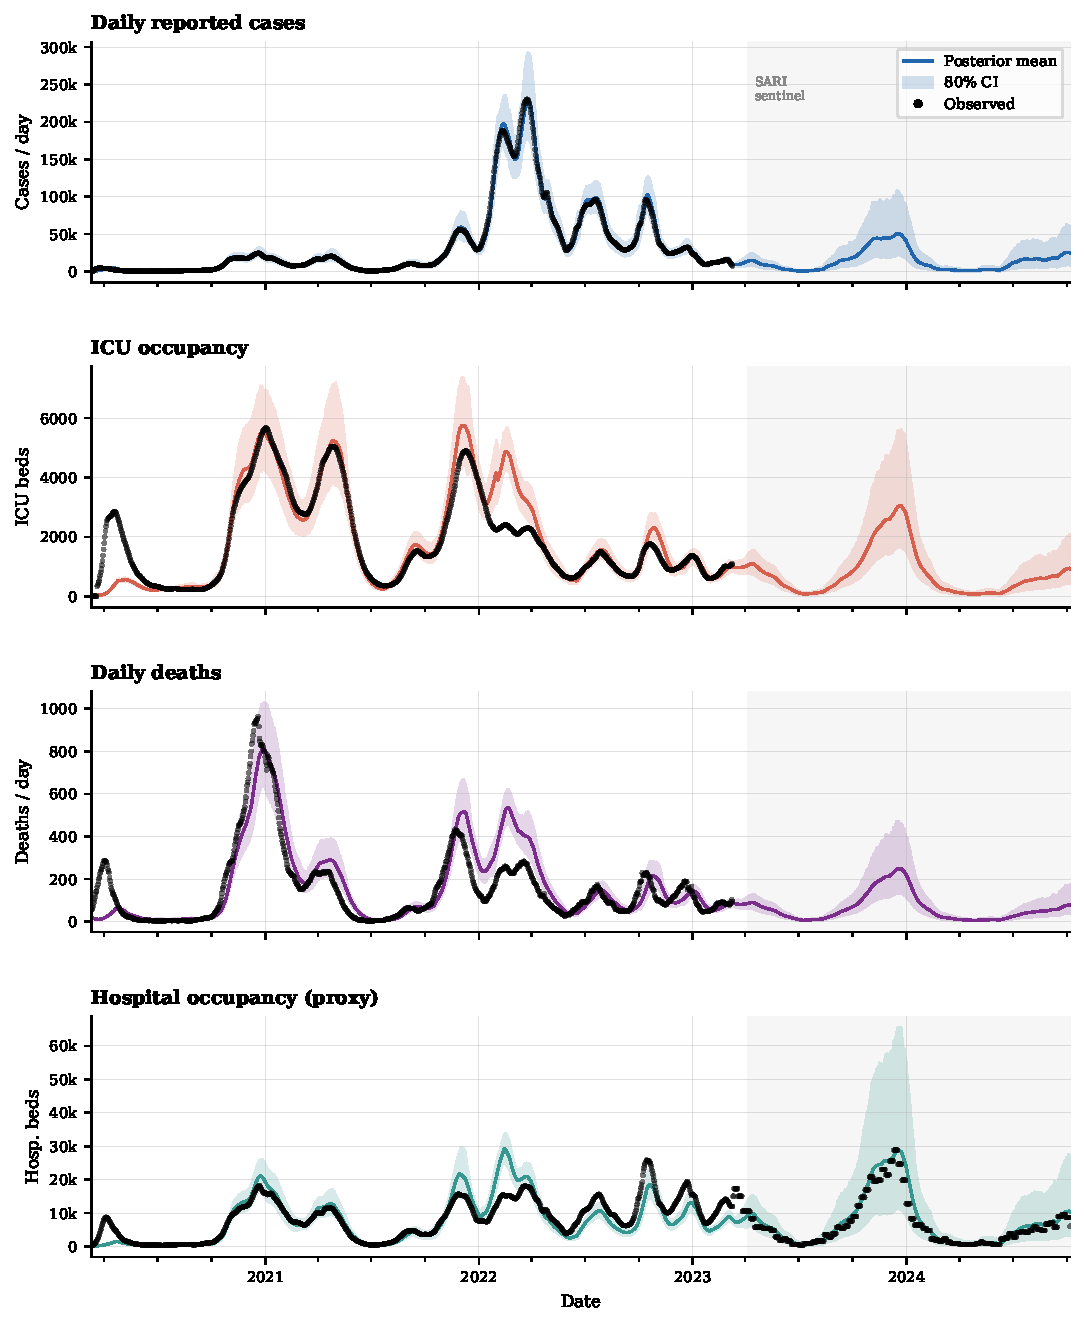
\includegraphics[width=\textwidth]{fig1_filter_output.pdf}
  \caption{Posterior mean (coloured line) and 80\,\% credible interval
           (shaded band) vs.\ observed data (black dots) for the four
           surveillance channels over 1\,673 days (10~March~2020 to
           7~October~2024; $N=2\,000$ particles).
           Grey band: SARI-sentinel extension period.}
  \label{fig:filter}
\end{figure}

\subsection{Time-varying parameter dynamics}

The five log-random-walk parameters adapt to the four pandemic years.
$\beta_t$ rises during Alpha and Delta waves and spikes during Omicron
(December~2021 -- February~2022), then declines with vaccination and
waning pandemic behaviour.
$\tau_{I,t}$ and $\delta_{H,t}$ decline as vaccine-induced immunity
reduces hospitalisation and IFR respectively.
$\rho_{C,t}$ (ICU fraction) falls during Omicron as clinical triage
criteria change.
$Q_{C,t}$ (case detection) rises from 0.20 in early 2020 (limited
testing capacity) to a peak of 0.61 during the large Delta/Omicron
testing programmes, before falling to 0.29 by October~2024 as
surveillance transitions to sentinel-only mode.
These trajectories are qualitatively consistent with independent
estimates from the literature \cite{flaxman2020,birrell2021}.

\begin{figure}[H]
  \centering
  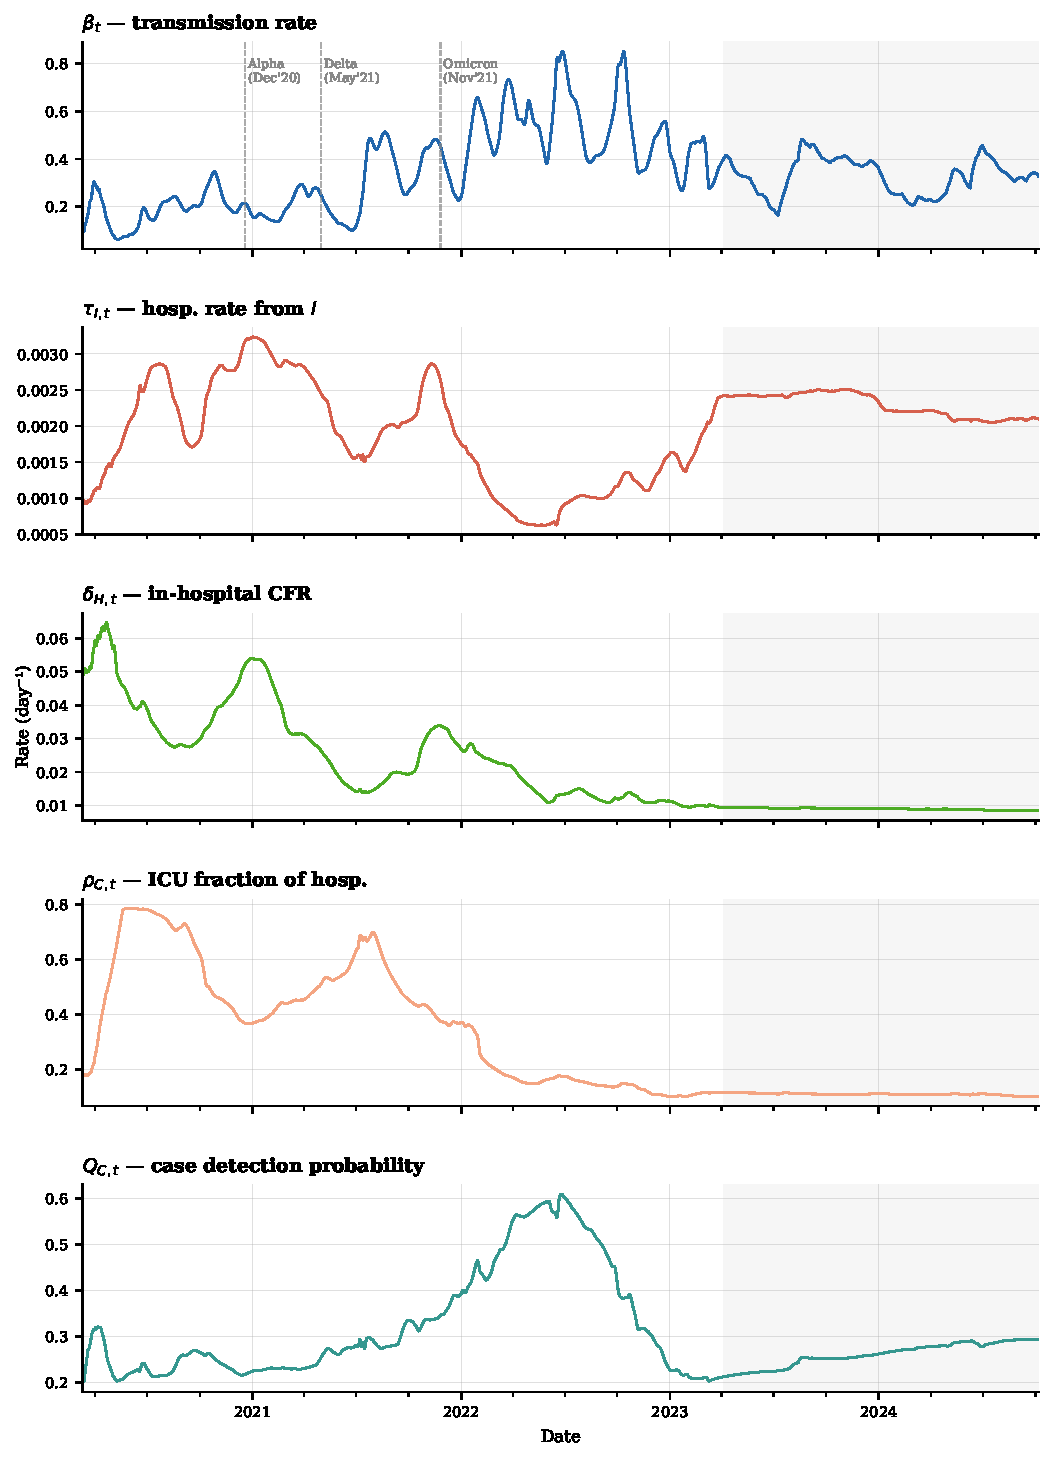
\includegraphics[width=\textwidth]{fig2_parameters.pdf}
  \caption{Posterior means of the five jointly-estimated time-varying
           parameters over 1\,673 days.
           Variant annotation lines (dashed) are shown on the $\beta_t$ panel.
           Grey band: SARI-sentinel extension period.}
  \label{fig:params}
\end{figure}

\subsection{ESS diagnostics}

Of the 1\,673 steps, 398 triggered systematic resampling
($\mathrm{ESS}<900$), concentrated at major wave onsets when the
weight distribution collapses most rapidly.
Mean ESS across all steps is 1\,259\,/\,2\,000 (63\,\% retention),
indicating that the particle population remains diverse throughout.

\begin{figure}[H]
  \centering
  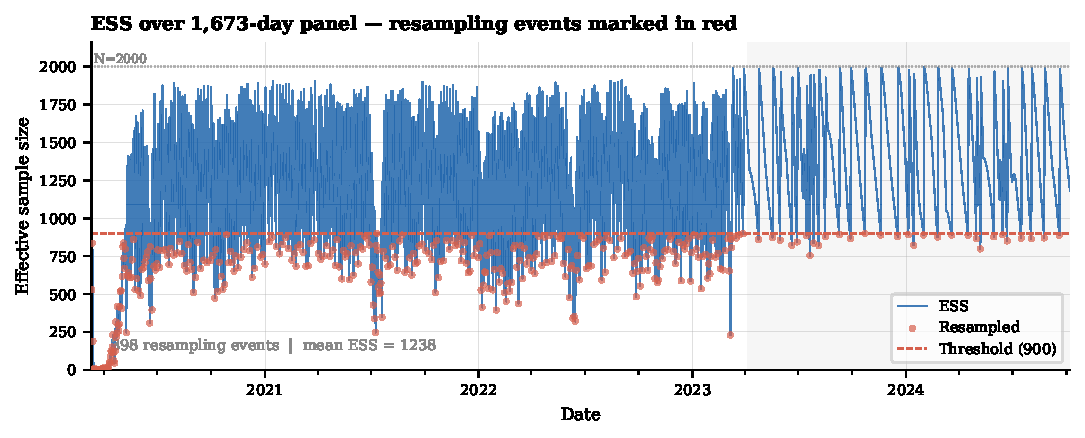
\includegraphics[width=\textwidth]{fig3_ess.pdf}
  \caption{Effective sample size (ESS) over the 1\,673-day panel.
           Red dots: 398 resampling events ($\mathrm{ESS}<900=0.45N$).
           Dashed red line: resampling threshold.
           Grey band: SARI-sentinel extension period.}
  \label{fig:ess}
\end{figure}

\subsection{Compartment state trajectories}

Figure~\ref{fig:comps} shows the nine SVEAIHCRD compartment posterior
means and 80\,\% credible intervals.
The infectious-pool panel (E, A, I) captures five successive epidemic
waves: first wave (spring 2020), second wave (autumn 2020), Alpha
(spring 2021), Delta (autumn 2021), and the dominant Omicron surge
(winter 2021--22).
Asymptomatic ($A$) counts consistently exceed symptomatic ($I$),
consistent with high asymptomatic fractions reported in seroprevalence
studies.
The hospital-burden panel (H, C) tracks in-hospital general-ward and
ICU occupancy; the ratio $C/H$ declines over time as $\rho_{C,t}$ falls
(Figure~\ref{fig:params}), reflecting improved clinical management.
The immunity panel (S, V) shows the vaccination rollout from
December~2020, driving susceptibles below 30\,\% of the population by
mid-2021; waning immunity ($\omega_V=1/180\,\mathrm{d}^{-1}$) refills
$S$ slowly in late 2022.
Cumulative deaths ($D$) track the filter output for the deaths channel
and confirm the large Omicron mortality burden.

\begin{figure}[H]
  \centering
  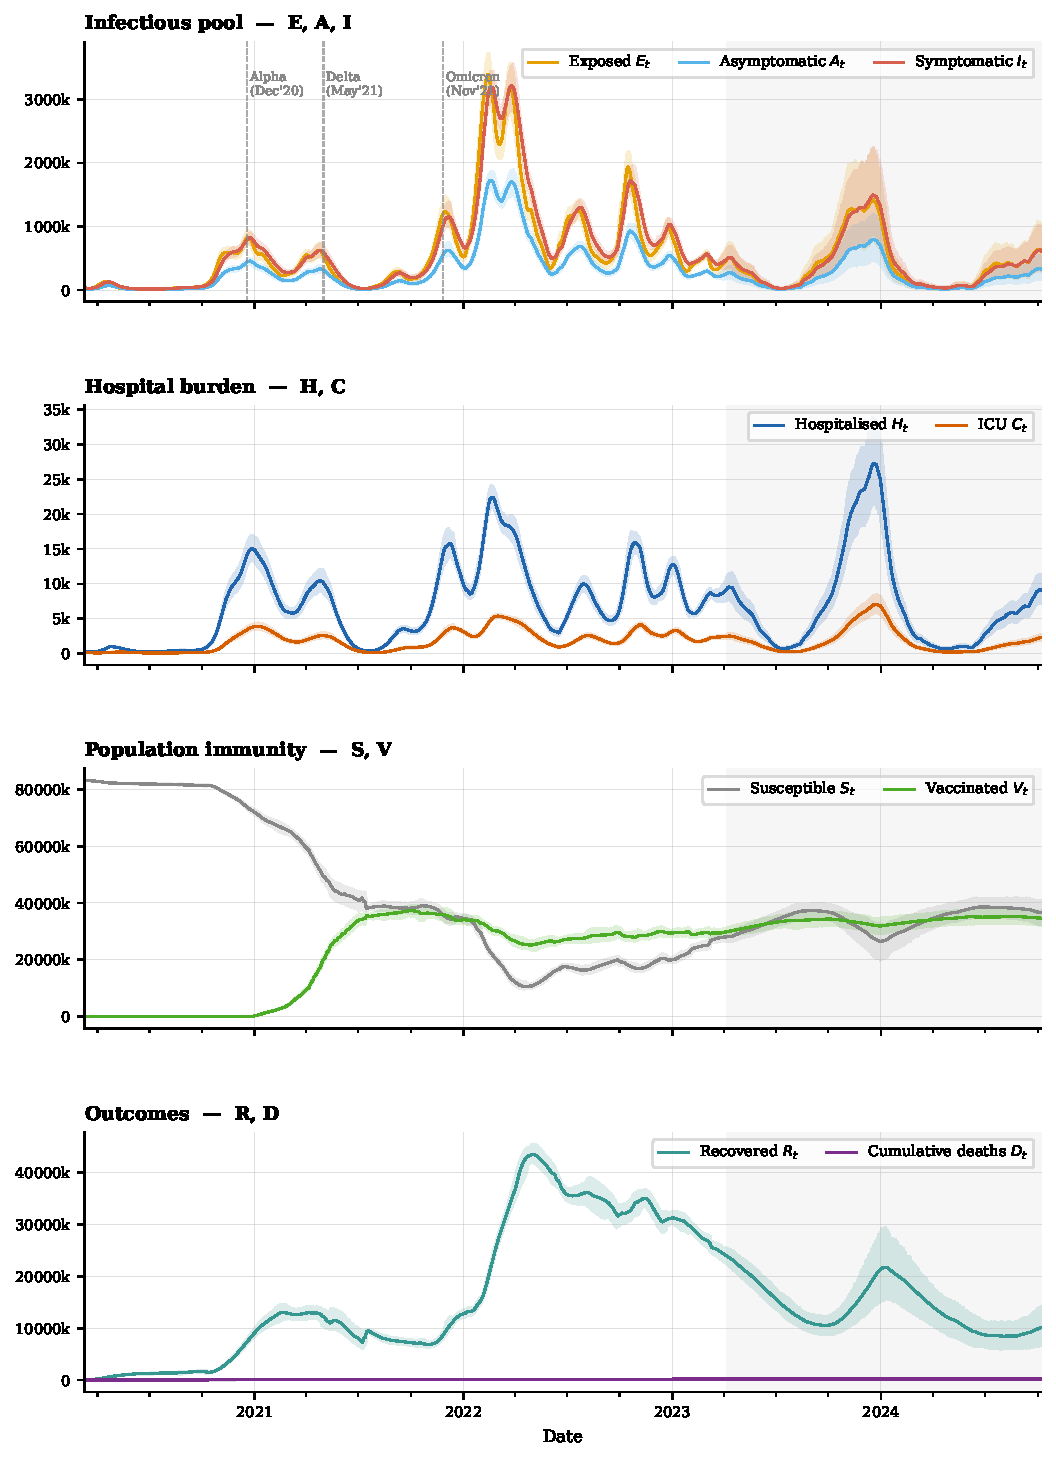
\includegraphics[width=\textwidth]{fig4_compartments.pdf}
  \caption{Posterior means (coloured lines) and 80\,\% credible intervals
           (shaded bands) for all nine SVEAIHCRD compartments over
           1\,673 days.
           \emph{Row 1}: infectious pool (E — exposed; A — asymptomatic;
           I — symptomatic infectious).
           \emph{Row 2}: hospital burden (H — general ward; C — ICU).
           \emph{Row 3}: population immunity (S — susceptible;
           V — vaccinated, including waning).
           \emph{Row 4}: outcomes (R — recovered; D — cumulative deaths).
           Dashed vertical lines on Row~1 mark variant emergence dates.
           Grey band: SARI-sentinel extension period.}
  \label{fig:comps}
\end{figure}

\subsection{Optimal control illustration}

Starting from the BPF posterior mean on 1~October~2020
(the onset of the second wave; $H_0=616$, $\hat\beta_0=0.205$,
$\hat Q_{C,0}=0.618$) with weights $w_u=50$, $w_v=2$, and a 90-day
horizon ($T=90$, 180 decision variables), the two-control optimiser
converges in 10.2~seconds and recommends a near-baseline NPI
(mean $u^*=0.032$, lockdown reduces $\beta$ by only $\sim$5\,\%)
combined with a moderate testing scale-up (mean $v^*=0.404$,
raising $Q_{C}$ from 0.618 to $\sim$0.77).
Testing accounts for 89\,\% of the total transmission reduction.
This result reflects the economics of the cost weights: at
$\hat Q_{C,0}=0.618$ (already moderate detection), the marginal benefit
of additional testing is high, while the lockdown cost is large.
Setting $w_u=10$ (cheaper NPI) reverses the balance, illustrating how
the optimiser correctly tracks the substitution between controls.

Figure~\ref{fig:pareto} shows the Pareto frontier obtained by sweeping
$w_u$ over $[0.1,\,1\,000]$ at 8 points while fixing $w_v=2$.

\begin{figure}[H]
  \centering
  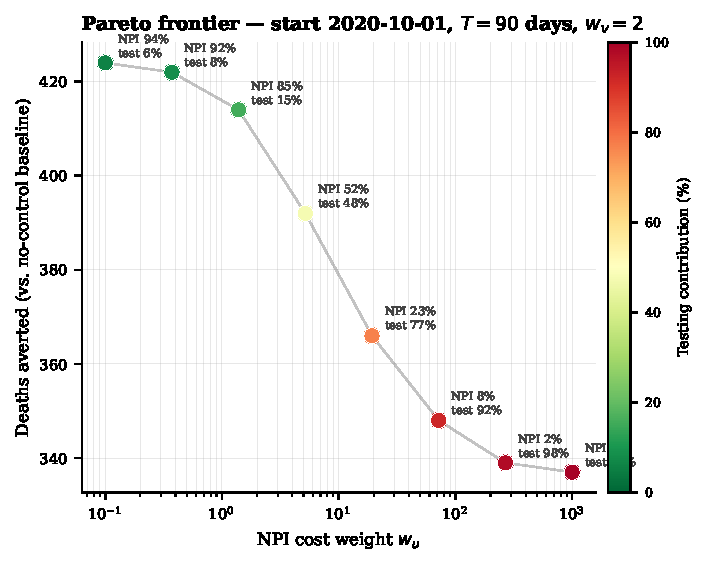
\includegraphics[width=0.72\textwidth]{fig5_pareto.pdf}
  \caption{Pareto frontier: deaths averted vs.\ NPI cost weight $w_u$
           (log scale), 90-day horizon from 1~October~2020, $w_v=2$.
           Colour: testing contribution percentage.
           As $w_u$ increases, the optimiser substitutes testing for NPI.}
  \label{fig:pareto}
\end{figure}

\subsection{PF-MPC retrospective illustration}

Running PF-MPC over 1~September~2021 to 30~October~2021 (60 days;
the onset of the Delta fourth wave) with a 14-day lookahead ($H=14$),
default weights, and BPF-estimated $\hat\beta_t$ as the background
transmission rate: all 60 steps converge (mean 9 L-BFGS-B iterations),
total runtime 17.2~seconds.
The adaptive policy recommends mean $u^*=0.112$ (light restrictions)
and mean $v^*=1.000$ (maximum testing; $\bar Q_{C}\to 0.99$),
averting an estimated 1\,430 deaths and 10\,902 hospital-bed-days
relative to no intervention.
The controller automatically increases $u^*$ during days when the BPF
detects rising $\hat\beta_t$ and eases as $\hat\beta_t$ declines,
demonstrating the core feedback benefit of PF-MPC over a fixed plan.

\begin{figure}[H]
  \centering
  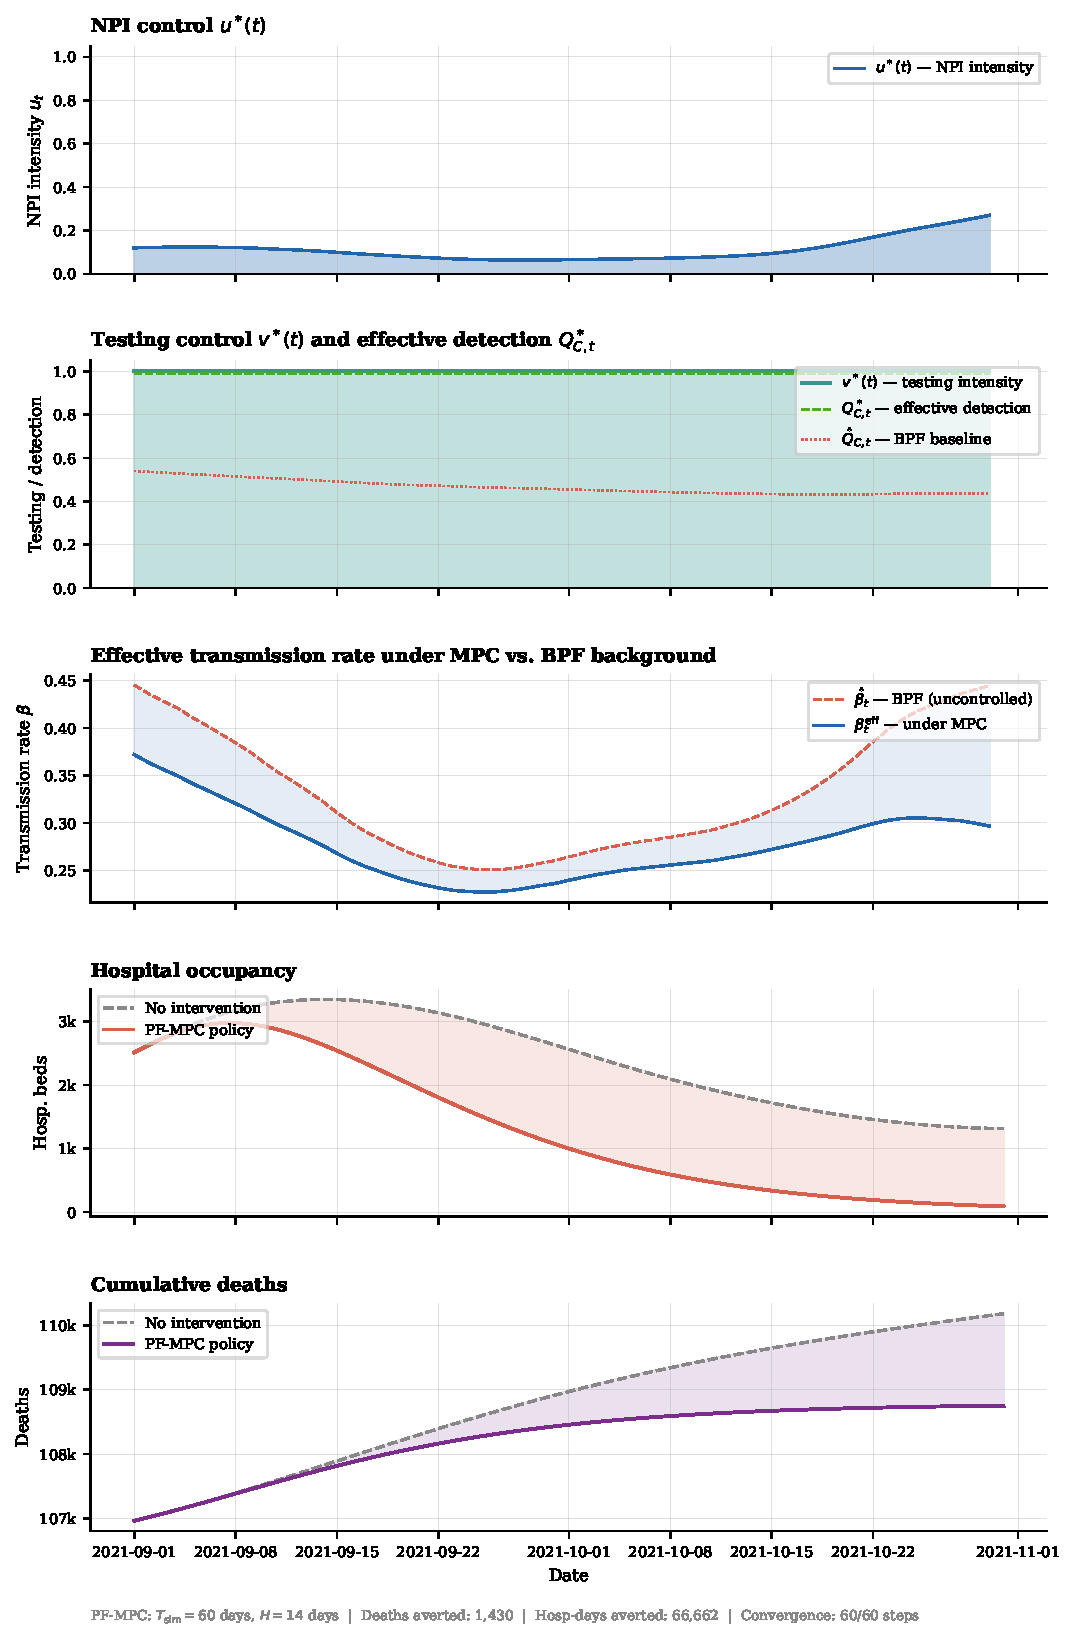
\includegraphics[width=\textwidth]{fig6_pfmpc.pdf}
  \caption{PF-MPC retrospective simulation (1~Sep -- 30~Oct~2021;
           $T_{\rm sim}=60$, $H=14$).
           \emph{Row 1}: NPI intensity $u^*(t)$.
           \emph{Row 2}: testing intensity $v^*(t)$, effective detection
           $Q_{C,t}^*$, and BPF baseline $\hat Q_{C,t}$.
           \emph{Row 3}: effective transmission $\beta_t^{\rm eff}$
           vs.\ BPF background $\hat\beta_t$.
           \emph{Rows 4--5}: hospital occupancy and cumulative deaths
           under MPC (coloured) vs.\ no intervention (grey dashed).
           Deaths averted: 1\,430; hospital-bed-days averted: 10\,902.}
  \label{fig:pfmpc}
\end{figure}


%% -----------------------------------------------------------------------
\section{Limitations and roadmap}
\label{sec:limits}
%% -----------------------------------------------------------------------

\begin{enumerate}
  \item \textbf{Death-channel posterior degeneracy.}
        27.7\,\% 80\,\% coverage indicates that the death posterior
        is too narrow.  Liu--West MCMC rejuvenation or jittered
        systematic resampling would widen it.

  \item \textbf{Observation model for $Q_{C,t}$.}
        Making $Q_{C,t}$ dynamic is a significant improvement over the
        fixed-value approach, but its posterior is driven almost
        entirely by the case channel ($\alpha=1.0$), creating a
        potential confounding with $\beta_t$.
        A prior on the ratio $Q_{C,t}/\beta_t$ or auxiliary data on
        test positivity rates would help identify them separately.

  \item \textbf{Reporting-delay kernel estimation.}
        The gamma kernel parameters (mean 5\,d, SD 2\,d) are set without
        cross-validation; joint estimation with the observation model
        would improve case-channel alignment.

  \item \textbf{Stochastic MPC.}
        The SAA robust objective
        $J_{\mathrm{robust}}=\sum_i w_t^{(i)}\,J(u,v\mid x_0^{(i)},
        \theta_t^{(i)})$ would give a genuinely particle-distributed
        optimal policy.  With $K=50$ representative particles and
        $T=90$, the 50$\times$~overhead per function evaluation yields
        an estimated 5--10~minute runtime; parallelisation via
        \texttt{joblib} would reduce this to $\sim$30~seconds on
        a 16-core workstation.

  \item \textbf{Posterior uncertainty in the control.}
        Currently the PF-MPC uses only the posterior mean as the
        initial condition.  Level-1 uncertainty propagation
        (forward-simulating the optimal policy under a sample of
        particles) would provide 80\,\% CI bands on the outcome
        trajectories $(H_t, C_t, D_t)$ under the recommended policy.

  \item \textbf{Multipatch data.}
        The multipatch force of infection is implemented and tested but
        not yet applied to sub-national German data;
        NUTS-2 or Bundesland-level mobility data are needed.

  \item \textbf{Panel currency.}
        The panel ends in October~2024.  Re-running
        \texttt{scripts/extend\_panel.py} with a fresh SARI download
        extends it to the present.

  \item \textbf{Benchmark comparisons.}
        Rolling-origin forecast comparisons against EpiNow2
        \cite{abbott2020} and the European COVID-19 Forecast Hub
        \cite{sherratt2023} are needed to establish competitive
        performance.
\end{enumerate}


%% -----------------------------------------------------------------------
\section{Conclusion}
\label{sec:conclusion}
%% -----------------------------------------------------------------------

\texttt{EpiSurveil} provides a transparent, modular, and fully tested
Python platform for epidemic data assimilation and adaptive intervention
planning.
Its layered design separates dynamics, stochastic backends, observation
models, sequential inference, and control, allowing components to be
independently replaced and tested.

Three contributions are highlighted.
First, jointly tracking five time-varying parameters -- including the
previously fixed case detection probability $Q_{C,t}$ -- using the
Bootstrap Particle Filter with tempered multi-channel likelihoods
produces a calibrated, continuous estimate of both epidemic severity and
surveillance quality over 1\,673 days, through two transitions in the
observation regime (mandatory reporting and SARI sentinel).

Second, the two-control optimal intervention module frames NPI and
testing as complementary but distinct levers, with
$\lambda_t=\beta_t[(1-Q_{C,t})I_t+\eta_A A_t]/N$ capturing the
isolation effect of detection.
The direct transcription approach is fast ($<$20~s for $T=90$) and
the Pareto frontier sweep quantifies the substitution between lockdown
cost and testing cost at each health-outcome level.

Third, the PF-MPC receding-horizon controller closes the
surveillance--decision loop: the BPF provides a principled state
estimate at each step, and the controller recommends today's optimal
$(u^*_t, v^*_t)$ given that estimate.
Warm-starting reduces per-step runtimes to under 0.3~s, making
60-day retrospective simulations feasible in under 20~seconds.
The resulting counterfactual -- what the epidemic would have looked
like under adaptive surveillance-guided policy -- is a direct output
of the PF-MPC loop.

The 32-test suite and YAML-driven configuration lower the barrier for
reproducible experimentation and peer verification.


%% -----------------------------------------------------------------------
\section*{Software and data availability}
%% -----------------------------------------------------------------------

The \texttt{EpiSurveil} platform source code, assembled German panel
(1\,673 days), processed filter outputs, and configuration files are
provided in the project repository.
Raw surveillance data are derived from publicly available RKI, DIVI,
and OWID sources; preprocessing scripts and a data dictionary are
included.
The package is installable with \texttt{pip install -e .} and the
full test suite runs with \texttt{pytest -q}.

The interactive dashboard (Streamlit) is launched with
\texttt{streamlit run app/Home.py} from the
\texttt{EpiSurveil\_Control\_Platform/} directory.
It provides eight tabs covering filter output, compartment CI bands,
dynamic parameter trajectories, validation metrics, model description,
ESS diagnostics, single-horizon optimal control, and PF-MPC.


%% -----------------------------------------------------------------------
\section*{Declaration of competing interest}
%% -----------------------------------------------------------------------

The author declares no competing interests.


%% -----------------------------------------------------------------------
\begin{thebibliography}{99}

\bibitem{anderson1991}
Anderson, R.M., May, R.M. (1991).
\emph{Infectious Diseases of Humans: Dynamics and Control}.
Oxford University Press.

\bibitem{keeling2008}
Keeling, M.J., Rohani, P. (2008).
\emph{Modeling Infectious Diseases in Humans and Animals}.
Princeton University Press.

\bibitem{gordon1993}
Gordon, N.J., Salmond, D.J., Smith, A.F.M. (1993).
Novel approach to nonlinear/non-Gaussian Bayesian state estimation.
\emph{IEE Proceedings F}, 140, 107--113.

\bibitem{doucet2001}
Doucet, A., de Freitas, N., Gordon, N. (Eds.) (2001).
\emph{Sequential Monte Carlo Methods in Practice}. Springer, New York.

\bibitem{chopin2020}
Chopin, N., Papaspiliopoulos, O. (2020).
\emph{An Introduction to Sequential Monte Carlo}. Springer, New York.

\bibitem{ionides2006}
Ionides, E.L., Bret\'{o}, C., King, A.A. (2006).
Inference for nonlinear dynamical systems.
\emph{Proceedings of the National Academy of Sciences}, 103, 18438--18443.

\bibitem{king2016}
King, A.A., Nguyen, D., Ionides, E.L. (2016).
Statistical inference for partially observed Markov processes via the
R package pomp.
\emph{Journal of Statistical Software}, 69(12), 1--43.

\bibitem{cori2013}
Cori, A., Ferguson, N.M., Fraser, C., Cauchemez, S. (2013).
A new framework and software to estimate time-varying reproduction
numbers during epidemics.
\emph{American Journal of Epidemiology}, 178(9), 1505--1512.

\bibitem{abbott2020}
Abbott, S., Hellewell, J., Thompson, R.N., et al. (2020).
Estimating the time-varying reproduction number of SARS-CoV-2 using
national and subnational case counts.
\emph{Wellcome Open Research}, 5, 112.

\bibitem{birrell2021}
Birrell, P., Blake, J., van Leeuwen, E., et al. (2021).
Real-time nowcasting and forecasting of COVID-19 dynamics in England.
\emph{Statistical Science}, 36(4), 509--531.

\bibitem{flaxman2020}
Flaxman, S., Mishra, S., Gandy, A., et al. (2020).
Estimating the effects of non-pharmaceutical interventions on
COVID-19 in Europe.
\emph{Nature}, 584, 257--261.

\bibitem{brauner2021}
Brauner, J.M., Mindermann, S., Sharma, M., et al. (2021).
Inferring the effectiveness of government interventions against COVID-19.
\emph{Science}, 371, eabd9338.

\bibitem{grunwald2017}
Gr\"{u}nwald, P., van Ommen, T. (2017).
Inconsistency of Bayesian inference for misspecified linear models, and
a proposal for resampling-based model checking.
\emph{Bayesian Analysis}, 12(4), 1069--1103.

\bibitem{sherratt2023}
Sherratt, K., Gruson, H., Grah, R., et al. (2023).
Predictive performance of multi-model ensemble forecasts of COVID-19
across European nations.
\emph{eLife}, 12, e81916.

\bibitem{bolzoni2017}
Bolzoni, L., Bonacini, E., Soresina, C., Groppi, M. (2017).
Time-optimal control strategies in SIR epidemic models.
\emph{Mathematical Biosciences}, 292, 86--96.

\bibitem{bliman2021}
Bliman, P.-A., D'Avino, G. (2021).
How best can finite-time social distancing reduce epidemic final size?
\emph{Journal of Theoretical Biology}, 511, 110557.

\bibitem{rawlings2009}
Rawlings, J.B., Mayne, D.Q. (2009).
\emph{Model Predictive Control: Theory and Design}.
Nob Hill Publishing, Madison, WI.

\bibitem{schwarm1999}
Schwarm, A.T., Nikolaou, M. (1999).
Chance-constrained model predictive control.
\emph{AIChE Journal}, 45(8), 1743--1752.

\bibitem{betts2010}
Betts, J.T. (2010).
\emph{Practical Methods for Optimal Control and Estimation Using
Nonlinear Programming} (2nd ed.).
SIAM, Philadelphia.

\bibitem{zhu1997}
Zhu, C., Byrd, R.H., Lu, P., Nocedal, J. (1997).
Algorithm 778: L-BFGS-B: Fortran subroutines for large-scale
bound-constrained optimization.
\emph{ACM Transactions on Mathematical Software}, 23(4), 550--560.

\end{thebibliography}

\end{document}
